\documentclass{article}
\usepackage{enumerate}
\usepackage{amsmath}
\usepackage{amssymb}
\usepackage{graphicx}
\usepackage{subfigure}
\usepackage{geometry}
\usepackage{color}
\usepackage{bm}
\usepackage{indentfirst}
\usepackage{array}
\usepackage{multirow}
\usepackage{diagbox}

\begin{document}

\vspace*{0.25cm}

\hrulefill

\thispagestyle{empty}

\begin{center}
\begin{large}
\sc{UM--SJTU Joint Institute \vspace{0.3em} \\ Physics Laboratory \\(VE215)}
\end{large}

\hrulefill

\vspace*{5cm}
\begin{Large}
\sc{{Laboratory Report}}
\end{Large}

\vspace{2em}

\begin{large}
\sc{{Exercise 4
\vspace{0.5em}

AC Lab
}}
\end{large}
\end{center}


\vfill

\begin{table}[h!]
\flushleft
\begin{tabular}{lll}
Name: Yihao Liu \hspace*{2em}&
ID: 515370910207\hspace*{2em}\\


\\

Date: 10 Nov 2016 

\end{tabular}
\end{table}

\hfill
\begin{tiny}
[rev. 1.0]
\end{tiny}
\newpage


\section{Goal}
\begin{enumerate}
\item
Learn how to define, calculate, and measure the amplitude of a sinusoidal
signal
\item
Learn how to define, calculate, and measure the Rise Time and Fall Time of a
signal
\item
Learn how to observe FFT spectra of signal and measure their parameters with
cursors
\item
Measure the waveforms and FFT spectra of various signals
\item
Compare your theoretical results obtained in the Pre-Lab with your In-Lab
data.
\end{enumerate}

\section{Introduction}

\subsection{High-Z mode}
Here I want to introduce you what is the High-Z mode we have kept emphasizing
during the previous Labs.

You have already learnt Thevenin equivalent of a circuit. You can think the
function generator in terms of its Thevenin equivalent circuit, which includes the
voltage source and $V_S$ and the equivalent resistance of 50 $\Omega$ as shown below.

\begin{figure}[!h]
	\centering
	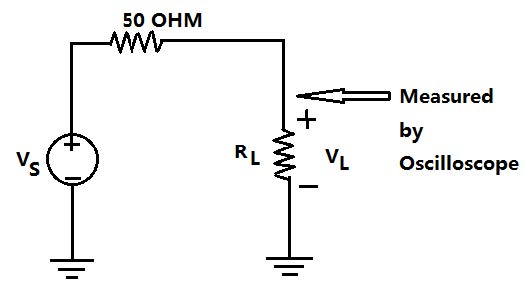
\includegraphics[width=10cm]{p1.jpg}
	\label{fig-1}
\end{figure}

When the load $R_L$ is 50 $\Omega$ , according to voltage division, we know that the VL
measured will be 0.5$V_S$. In this case, we use the 50 OHM mode, in which the
function generator produces voltage $V_S$ but displays voltage 0.5$V_S$. In that way, if
you set 2$V_{ppk}$ for the function generator, the actual $V_S$ will be 4$V_{ppk}$ to make sure
the load get a voltage of 2$V_{ppk}$.

In our lab measurements, the load resistance $R_L$ is very high—the input resistance
of the oscilloscope is about 1 $M\Omega$ . The $V_L$ measured across $R_L$ practically equals
$V_S$. So we use High Z mode, in which the function generator produce voltage $V_S$
and displays $V_S$.

\subsection{The Rise Time and Fall Time of signals}

The Rise time is the interval between the moment of the time when the signal
reaches its 10\% level and the moment of time when the signal reaches its 90\%.
We have already used this concept in our Lab3.

\begin{figure}[!h]
	\centering
	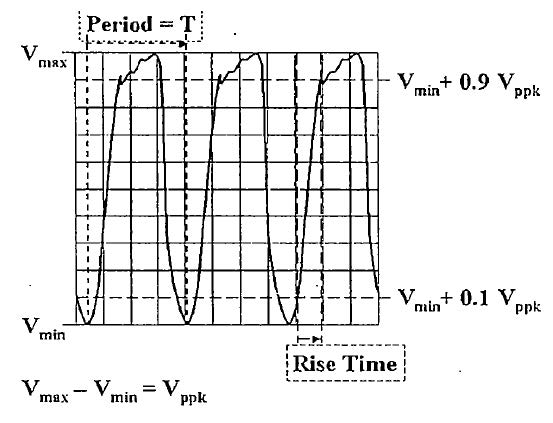
\includegraphics[width=10cm]{p2.jpg}
	\label{fig-2}
\end{figure}

\begin{figure}[!h]
	\centering
	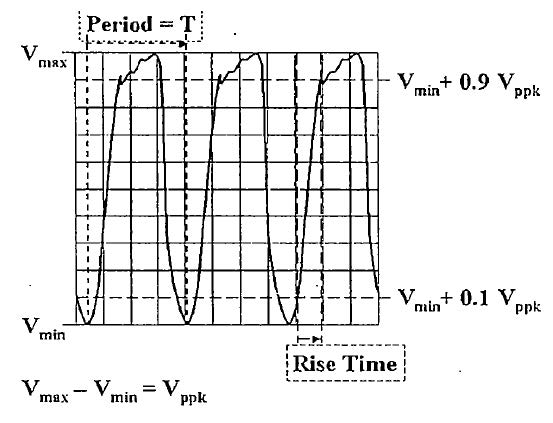
\includegraphics[width=10cm]{p2.jpg}
	\label{fig-3}
\end{figure}

The above two figures illustrate the rise time of a sinusoidal like wave and a
saw-tooth wave. If you do not know what is $V_{ppk}$, you can refer to part 4 of this
section.

Take the sinusoid wave as an example to calculate the rise time.

$$y=\frac{V_{ppk}}{2}\sin(2\pi ft)$$

$$V_{min}=\frac{-V_{ppk}}{2},V_{max}=\frac{V_{ppk}}{2}$$

$$Rise\ Time=\frac{\arcsin\left(\frac{V_{min}+0.9V_{ppk}}{0.5V_{ppk}}\right)-\arcsin\left(\frac{V_{min}+0.1V_{ppk}}{0.5V_{ppk}}\right)}{2\pi f}$$


\subsection{Fourier Series Representation of a Signal}

Here I am going to give you a general idea of Fourier Series to help you
understand some parts of this lab. You will learn Fourier Series in details in your
math course this semester.

Fourier series is a way to represent a wave-like function as a combination of
simply sine waves. It decomposed and period function into the sum of a (possibly
infinite) set of simple oscillation functions.

Let $x(t)$ be a periodic signal with fundamental period $T_0$. It can be represent by the following synthesis equation,

$$x(t)=\sum_{k=-\infty}^{\infty}c_ke^{jk\omega_0t}, {\rm where} \omega_0=\frac{2\pi}{T_0}$$

The coefficients $c_k$ in the above equation can be calculated by the analysis
equation,

$$C_k=\frac{1}{T_0}\int_0^{T_0}x(t)e^{-jk\omega_0t}dt,k=0,\pm 1,...$$

\subsection{Four ways to measure the amplitude of a sinusoid}

\begin{enumerate}[a)]
\item
$\rm V_{peak}=V_p=V_{pk}=V_0$ is the peak amplitude of the sinusoid measured in V or mV.
\item
$\rm V_{peak-to-peak}=V_{ppk}=V_{max}-V_{min}=2V_0$ is the value we often use in the lab to
determine the overall size of the waveform. We have used it many times in the previous Labs.
\item
$\rm V_{RMS}$ is the Root-Mean-Square, or RMS amplitude of the sinusoid. The
sinusoidal voltage $V=V_0\sin(\omega t+\theta)$ dissipates as much power in the load resistor
as does the DC voltage equals to $V_{RMS}$

\begin{figure}[!h]
	\centering
	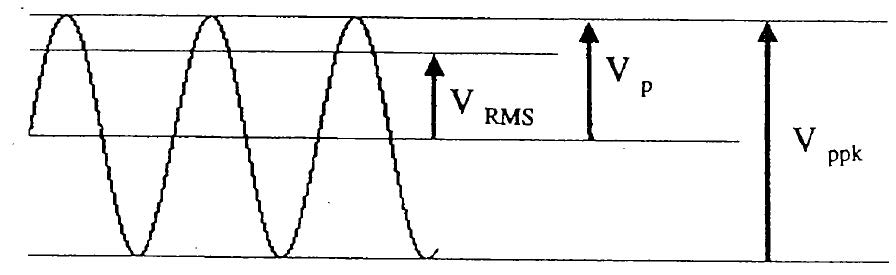
\includegraphics[width=10cm]{p4.jpg}
	\label{fig-4}
\end{figure}

For any periodic function f(t) that has period T, the RMS amplitude is defined as

$$Amplitude,RMS=\sqrt{\frac{1}{T}\int_{t_0}^{t_0+T}f^2(t)dt}$$

In the case of sinusoid $f(t)=V_0\sin(\omega t+\theta)$,

$$V_{RMS}=\frac{V_0}{\sqrt{2}}=\frac{V_{peak}}{\sqrt{2}}=\frac{V_{ppk}}{2\sqrt{2}}$$

\item

The above three ways all study the signal in time domain, plotted as voltage vs.
time. In this Lab, we also need to study the frequency domain, when you measure
their spectra displayed as amplitude vs. frequency. In frequency domain, the
oscilloscope measures the amplitude of on a logarithmic scale, using decibels.

$$Amplitude\ in\ decibels(dBv)=20\log\left(\frac{Amplitude\ in\ V_{RMS}}{1V_{RMS}}\right)$$

Decibels are used to calculate ratios of two amplitudes on a logarithmic scale.

$$Ratio,in\ decibels(dB)=20\log\left(\frac{Amplitude\ of\ signal\ \sharp 2,RMS}{Amplitude\ of\ signal\ \sharp 1,RMS}\right)$$

\end{enumerate}

\section{In-Lab Procedure}

\subsubsection{Part 1}

\begin{enumerate}
\item
On the function generator, set a sine wave at 1 [kHz] and keep its amplitude
at 3 [Vpp]. The load must be High-Z mode.
\item
Record the parameters on the datasheet. Fill the table with the data set on the
function generator and displayed on the oscilloscope.
\item
Repeat the Step 2 with a sine wave at 1.5 [kHz] and 5 [Vpp] on the function
generator. The load should remain High-Z mode.
\item
In post-report, calculate the rise time in theory and compare it with the values
displayed on the oscilloscope.
\end{enumerate}

\subsubsection{Part 2}

\begin{enumerate}
\item
First, we set a sine wave and a square wave, respectively. The frequency is 1
[kHz] and the amplitude is 3 [Vpp].
\item
On the oscilloscope, set 1 [V/div] and 5 [ms/div].
\item
Push the “MATH” button and select “FFT” function.
\item
Push the “cursor” button and select “trace” mode to trace the spectrum.
\item
When the cursor reach a peak of the spectrum, record the Frequency in [kHz]
and the Amplitude in [dBV].
\item
Set another sine wave and a square wave. The frequency is 2 [kHz] and the
amplitude is 6 [Vpp]. Repeat the steps above.
\item
In post-report, you need to calculate the theoretical amplitude of sine wave in
[dBV]. Besides, you need to calculate the Vpeak of each square wave
measured in Part II. You should give a brief conclusion on what you learn
from this lab.
\end{enumerate}

\section{Results and Discussion}

\subsection{Part 1}

\begin{table}[!h]
\begin{center}
\begin{tabular}{|c|c|c|}
\hline
 & Set on Function Generator & Measured with Oscilloscope \\
\hline
Amplitude in Vpp [V] 	&	3.00	&	3.10	\\
\hline
Frequency [kHz]			&	1.000	&	0.999	\\
\hline
Rise Time [$\mu$s]		&	295.2	&	292	\\
\hline
Amplitude in Vpp [V] 	&	5.00	&	5.16	\\
\hline
Frequency [kHz]			&	1.500	&	1.499	\\
\hline
Rise Time [$\mu$s]		&	196.8	&	199	\\
\hline
\end{tabular}
\caption{Rise Time Measurement.}
\label{tab-1}
\end{center}
\end{table}

For the 3V Vpp,

$$t=292\,\rm \mu s$$

Theoretically,

$$t=\frac{\arcsin\left(\frac{V_{min}+0.9V_{ppk}}{0.5V_{ppk}}\right)-\arcsin\left(\frac{V_{min}+0.1V_{ppk}}{0.5V_{ppk}}\right)}{2\pi f}=295.2\,\rm \mu s$$

The relative error is $1.1\%$\\

For the 5V Vpp,

$$t=199\,\rm \mu s$$

Theoretically,

$$t=\frac{\arcsin\left(\frac{V_{min}+0.9V_{ppk}}{0.5V_{ppk}}\right)-\arcsin\left(\frac{V_{min}+0.1V_{ppk}}{0.5V_{ppk}}\right)}{2\pi f}=196.8\,\rm \mu s$$

The relative error is $1.1\%$\\

We can find that relative error is very small.

\subsection{Part 2}

\subsubsection{Set the wave at 3 [Vpp] 1 [kHz]}

\begin{table}[!h]
\begin{center}
\begin{tabular}{|c|c|c|}
\hline
Peak & Frequency (measured) [kHz] & Amplitude (measured) [dBV] \\
\hline
$f_0$ &	1.000	&	0.16	\\
\hline
\end{tabular}
\caption{FFT spectrum for Sine wave.}
\label{tab-2}
\end{center}
\end{table}

$$A_{dBV}=0.16$$

Theoretically,

$$A_{dBV}=20\log\left(\frac{A_{RMS}}{1V_{RMS}}\right)=0.51$$

The relative error is $218.8\%$\\


\begin{table}[!h]
\begin{center}
\begin{tabular}{|c|c|c|}
\hline
Peak & Frequency (measured) [kHz] & Amplitude (measured) [dBV] \\
\hline
$f_0$  &	1.000	&	1.76	\\
\hline
$3f_0$ &	3.000	&	-5.28	\\
\hline
$5f_0$ &	5.000	&	-8.16	\\
\hline
$7f_0$ &	6.996	&	-10.4	\\
\hline
$9f_0$ &	9.008	&	-10.4	\\
\hline
\end{tabular}
\caption{FFT spectrum for Square wave.}
\label{tab-3}
\end{center}
\end{table}




\subsubsection{Set the wave at 6 [Vpp] 2 [kHz]}

\begin{table}[!h]
\begin{center}
\begin{tabular}{|c|c|c|}
\hline
Peak & Frequency (measured) [kHz] & Amplitude (measured) [dBV] \\
\hline
$f_0$ &	5.000	&	5.60	\\
\hline
\end{tabular}
\caption{FFT spectrum for Sine wave.}
\label{tab-4}
\end{center}
\end{table}

$$A_{dBV}=5.6$$

Theoretically,

$$A_{dBV}=20\log\left(\frac{A_{RMS}}{1V_{RMS}}\right)=6.53$$

The relative error is $16.6\%$\\


\begin{table}[!h]
\begin{center}
\begin{tabular}{|c|c|c|}
\hline
Peak & Frequency (measured) [kHz] & Amplitude (measured) [dBV] \\
\hline
$f_0$  &	2.000	&	1.76	\\
\hline
$3f_0$ &	6.020	&	-1.20	\\
\hline
$5f_0$ &	10.020	&	-5.20	\\
\hline
$7f_0$ &	14.000	&	-6.00	\\
\hline
$9f_0$ &	18.000	&	-8.40	\\
\hline
\end{tabular}
\caption{FFT spectrum for Square wave.}
\label{tab-5}
\end{center}
\end{table}


\section{Conclusion}
In the lab, we learn how to define, calculate, and measure the amplitude of a sinusoidal
signal. We
learn how to define, calculate, and measure the Rise Time and Fall Time of a
signal. We
learn how to observe FFT spectra of signal and measure their parameters with
cursors.
We
measure the waveforms and FFT spectra of various signals

We compare the theoretical results obtained in the Pre-Lab with the In-Lab
data.

\section{Reference}
Lab 4 Manual.

\section{Pre-lab and Data sheet}

\end{document}